由于我们并不是先实现了另外的模型再在此基础上进行改进,而是直接对我们的模型进行设计和搭建的,所以在本部分的内容中,我们将对于我们的模型结构和设计思路进行详细的介绍。
\subsection{模型结构}
模型结构图如图9所示。
\begin{figure}[htb]        
\center{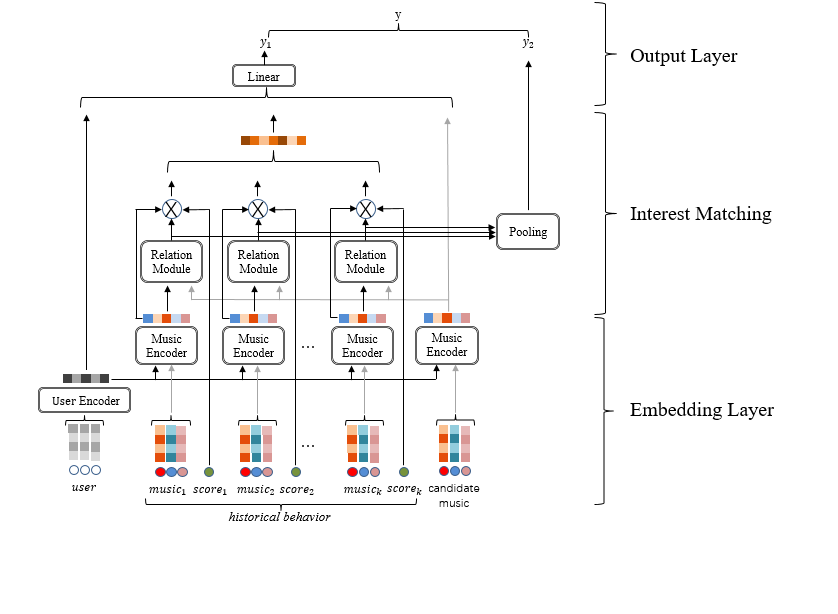
\includegraphics[width=15cm]  {MusicRecomSurvey/pics/model_final.PNG}}    
\caption{\label{4} 模型结构图}      
\end{figure}

\subsubsection{Embedding Layer}
根据我们的数据集,我们可以获得若干的特征,我们将特征先通过线性层或者Embeding层进行编码,得到一系列特征的向量表示。接下来就是根据这些向量,对于用户及音乐进行编码。下方的user表示目标用户的若干特征,用向量表示。将其作为输入,经过User Encoder,得到对于用户特征的编码向量。接下来,对于一些用户已经评分过的音乐,我们知道这些音乐的特征和评分,我们将特征和用户的特征向量结合在一起,分别输入到Music Encoder中进行编码,此时能够结合用户对于音乐的个性化信息,从而相同的音乐对于不同的用户来讲,经过Music Encoder得到的编码是不同的。对于待评价的音乐,我们只有他们的特征值,但是仍然可以像已知评价的音乐那样,通过Music Encoder,获得其特征向量。这部分就是音乐的编码层Embedding Layer。具体地,两种Encoder的结构如图10所示,可以见到Encoder的主要结构是Multi-Head Attention\cite{vaswani2017attention}模块,其结构如图11所示。

关于音乐选取的数量,我们也进行了一定的调整。我们在输入时需要有一系列已知评分的特征以及其最终的评分,但是一个人的历史记录会有很多条,并且数量各不相同,而我们的模型结构并不支持对于输入数量动态进行调整,所以我们选择使用采样的方法,每次训练时,从用户的历史音乐中选取5首历史评价过的歌曲进行输入,经过多轮训练后,基本能够将所有的评价歌曲均利用在训练当中。这种方法虽然对数据集的利用效率不高,但是能够较大地降低训练的时间成本和模型的复杂度,所以我们经过权衡,选择了随机选取5条数据的方法。

\begin{figure}[htbp]        
\center{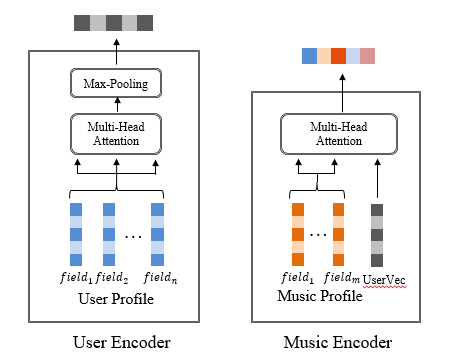
\includegraphics[width=10cm]  {MusicRecomSurvey/pics/model_encoder.PNG}}    
\caption{\label{4} Encoder结构}      
\end{figure}

\begin{figure}[htbp]        
\center{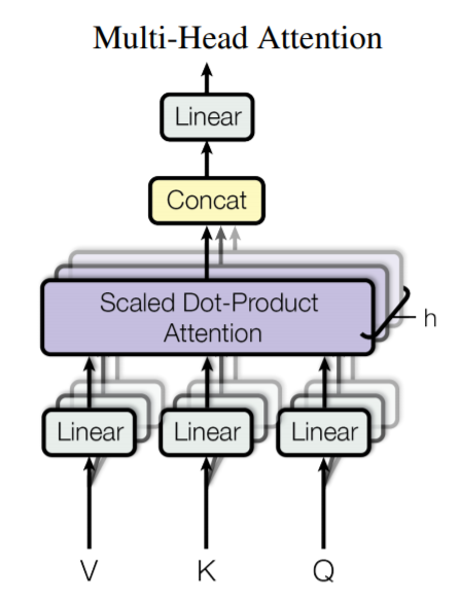
\includegraphics[width=7cm]  {MusicRecomSurvey/pics/Multihead.png}}    
\caption{\label{4} Multi-Head结构}      
\end{figure}


\subsubsection{Interest Matching}
\begin{figure}[htbp]        
\center{
\includegraphics[width=7cm]  {MusicRecomSurvey/pics/relation_module.png}}    
\caption{\label{4} Relation Module结构}      
\end{figure}

之后我们根据若干已评价的音乐和一个待评价音乐的特征向量,通过一个Relation Module,具体结构如图12所示。通过这样的结构,可以对于这些音乐之间的相似度进行预测,其得到的结果就是已知评分音乐和未知评分音乐之间的相似程度。事实上,我们的Relation Module并不算特别复杂,需要训练的参数只有一个矩阵$W$,事实上,我们也使用更加深层的结构替换本结构进行了测试,但是发现这样做不仅会增加训练时间和参数规模,并且得到的准确度也会下降一些,所以最终我们还是选择了将两向量关于$W$求内积之后再进行$sigmoid$得到0\~1之间的值作为相似程度。

根据相似度,我们将根据已知评分音乐的相关特征,构造处待预测音乐的特征。方法就是加权平均,每一项的权值是得分乘上相似度,从而,越相似的音乐,以及得分越高的音乐,对于预测结果的影响就越明显。最后得到特征向量的一个估计值。

\subsubsection{Output Layer}
最后就是一个Output Layer输出层,综合之前给出的两项评分结果,给出最后的结论。第一部分的结论$y_1$有由之前的用户编码,待预测音乐估计特征,待预测音乐编码等内容过一个线性层,得到的结果,这部分体现处了协同过滤思想中根据相似度和评分得到目标评分的思想。另一部分结论$y_2$得到的方法是通过一个Max Pooling层,选取出相关性最大的值。这部分体现出的策略是当待预测歌曲和之前的历史歌曲有很高的相似性时,我们认为用户很有可能对于待评价歌曲有一定的兴趣,所以此时该结果是一个较大的相似度的值。最后,我们将两个评分制取平均,得到最终的输出。这是一个0\~1之间的值表示用户可能感兴趣的程度。

\subsection{模型创新点}
我们的模型对于这些问题进行了一定的讨论和修正。

首先,我们引入了Self Attention机制和Multi-head Attention机制\cite{vaswani2017attention},在编码层实现了用户个性化的音乐编码,即将用户的特征编码用于音乐的编码过程,这就保证了对于不同的用户,就算是相同的歌曲,其编码也是不同的。这就保证了推荐过程更加富有个性化。

此外,我们考虑了不同交互行为对于提取用户兴趣的不同贡献,给出了一套用户兴趣的评分系统,并在利用历史交互信息捕捉用户兴趣时,实现了对于特征的降噪处理。

同时,我们引入了比较学习的思路,基于比较用户以往喜欢的物品以及待判断物品的思路,挖掘深层次的特征,从而能够更好地捕捉用户兴趣。并最终取得了较好的实验结果,具体的结果比较将在后面的部分给出。